\chapter{Beschreibung einer Sicherheitsl\"ucke}
\label{chap:4}

Noch bevor eine endgültige Fassung des 5G-AKA Protokolls feststand haben sich einige Forscher bereits mit unterschiedlichen Sicherheitsaspekten des Protokolls auseinandergesetzt und teilweise sogar mögliche Sicherheitslücken entdeckt.
\textit{Martin Dehnel-Wild} und \textit{Cas Cremers} haben in \textit{Security vulnerability in 5G-AKA draft} solch eine Sicherheitslücke vorgestellt. %Security vulnerability in 5G-AKA draft
Ihre Befunde beziehen sich auf die Spezifikation TS 33.501 V0.7.0 des 3GPP. %3GPP TS 33.501 V0.7.0
mittlerweile hat das 3GPP bereits neuere Versionen der Spezifikation veröffentlicht, darunter auch die Version V15.34.1, auf der die Beschreibung aus \cref{chap:2} beruht. %3GPP TS 33.501 V15.34.1
Da sich zwischen den Versionen V0.7.0 und V15.34.1 vor allem die Benennung einiger Komponenten verändert hat, wird zur Verbesserung der Übersichtlichkeit im weiteren Verlauf die Sicherheitslücke im Kontext der Spezifikation TS 33.501 V15.34.1 beschrieben.


\section{Beschreibung der Sicherheitslücke}

\begin{figure}[H]
  \centering
  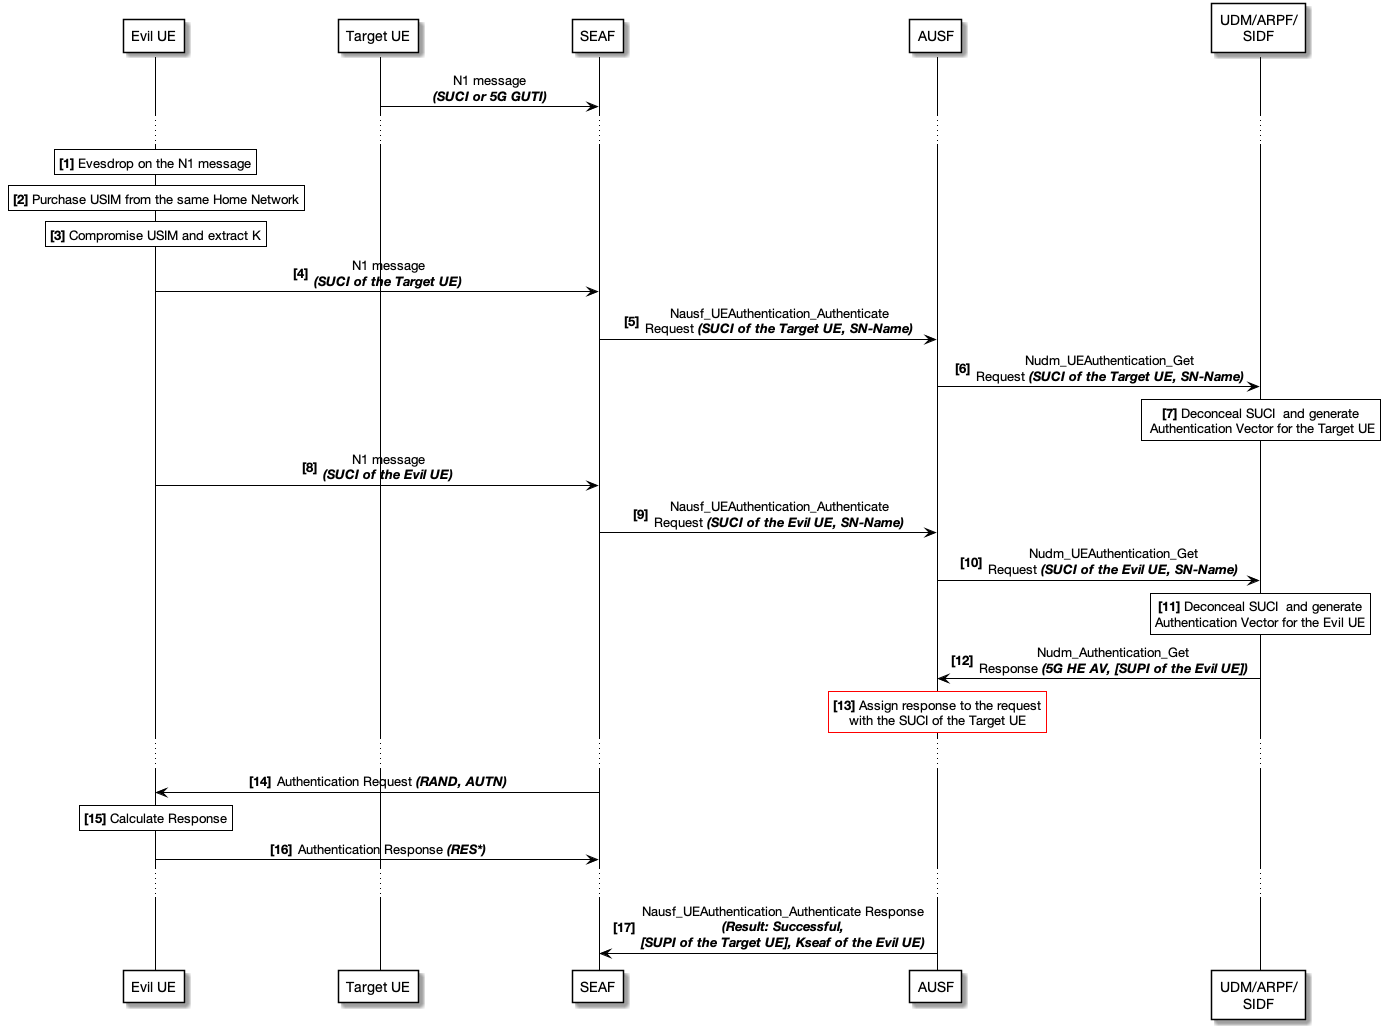
\includegraphics[width=\textwidth]{uml/vulnerability_v1.png}
  \caption{Erfolgreiche Authentifikation}
  \label{fig:protocol_v1}
\end{figure}

Die in \textit{Security vulnerability in 5G-AKA draft} vorgestellte Sicherheitslücke ermöglicht es einem Angreifer sich als ein anderer Benutzer auszugeben. %Security vulnerability in 5G-AKA draft
Zur Vereinfachung wird hier davon ausgegangen, dass das \gls{udm}/\gls{arpf}/\gls{sidf} immer das 5G-AKA Protokoll auswählt und nicht das EAP-AKA' Protokoll.
Damit dieser hier beschriebene Angriff erfolgreich ausgeführt werden kann müssen jedoch einige Vorbereitungen getroffen werden.

\subsection{Vorbereitungen}

\begin{enumerate}
\item Der Angreifer muss an den \gls{suci} des Benutzers kommen für den er sich ausgeben möchte.
Dafür muss er die \textit{N1 message} des Benutzers mithören und aufzeichnen.

\item Hat der Angreifer die \textit{N1 message} des Benutzers aufgezeichnet, dann bringt er in Erfahrung zu welchem \textit{Home Network} der \gls{suci} gehört und kauft sich ein legitimes \gls{usim} des selben \textit{Home Network}s.

\item Ist der Angreifer im Besitz des legitimen \gls{usim} so kompromittiert er dieses und extrahiert daraus den Langzeitschlüssel \gls{k}.

\end{enumerate}

\subsection{Der Hauptteil des Angriffs}

\begin{enumerate}
\setcounter{enumi}{3}

\item Der Angreifer sendet nun eine \textit{N1 message} an die \gls{seaf} und initiiert somit eine neue Authentifikation.
Diese Nachricht enthält den \gls{suci} des Benutzers, den der Angreifer in \textit{Schritt 1} abgehört hat.

\item Der \gls{suci} des abgehörten Benutzers wird von der \gls{seaf} an die \gls{ausf} weitergeleitet.

\item Das \gls{udm} erhält den \gls{suci} des abgehörten Benutzers und beginnt die erhaltene Nachricht zu verarbeiten.

\item Das \gls{udm} berechnet den \gls{supi} des abgehörten Benutzers aus dem \gls{suci} den es in \textit{Schritt 6} erhalten hat und generiert einen Authentifikations-Vektor für den \gls{suci} des abgehörten Benutzers.

\item Direkt nach dem versenden der Nachricht aus \textit{Schritt 4} sendet der Angreifer erneut eine \textit{N1 message} jedoch dieses mal mit dem \gls{suci} des \gls{usim}s das er in \textit{Schritt 2} gekauft hat.

\item Auch der \gls{suci} des Angreifers wird von der \gls{seaf} an die \gls{ausf} weitergeleitet.

\item Das \gls{udm} erhält den \gls{suci} des Angreifers kurz nachdem es den \gls{suci} des abgehörten Benutzers erhalten hat.

\item Das \gls{udm} berechnet den \gls{supi} des Angreifers aus dem \gls{suci}, den es in \textit{Schritt 9} erhalten hat und generiert den Authentifikations-Vektor  für den \gls{suci} des Angreifers.

\item Das \gls{udm} hat in \textit{Schritt 7 \& 11} erst den \gls{suci} des abgehörten Benutzers und dann den \gls{suci} des Angreifers erhalten.
Nun sendet es aber erst den Authentifikations-Vektor für den \gls{suci} des Angreifers an die \gls{ausf} zurück.
Das \gls{udm} sendet also die Antworten auf die erhaltenen Nachrichten nicht in der gleichen Reihenfolge zurück in der es die \gls{suci}s erhalten hat.

\item Die \gls{ausf} erhält nun zuerst die Antwort auf die Nachricht aus \textit{Schritt 11}.
Da die Antwort des \gls{udm} nicht den \gls{suci} enthält kann die \gls{ausf} nicht überprüfen zu welchem \gls{suci} die Antwort gehört und nimmt daher fälschlicherweise an, dass die erhaltene Antwort zur Nachricht aus \textit{Schritt 6} gehört.

\item In Schritt 14 erhält der Angreifer von der \gls{seaf} den Authentication Request.
Diese Nachricht enthält nun \gls{rand} und \gls{autn} die das \gls{udm} für den \gls{suci} des Angreifers, die \gls{seaf} jedoch nimmt an, das \gls{rand} und \gls{autn} für die Authentifizierung des abgehörten Benutzers bestimmt sind.

\item Der Angreifer kann nun \gls{res*} aus \gls{rand} und \gls{autn} berechnen, da er in \textit{Schritt 3} den dafür benötigten Langzeitschlüssel \gls{k} erhalten hat.

\item Der Angreifer sendet nun die in \textit{Schritt 15} berechnete \gls{res*} an die \gls{seaf}.

\item Die \gls{seaf} und die \gls{ausf} überprüfen nun die \gls{res*} aus \textit{Schritt 16} und akzeptieren sie schließlich.
Das 5G-AKA Protokoll wurde also erfolgreich ausgeführt.
Jedoch nehmen \gls{seaf} und \gls{ausf} an, dass sich der abgehörte Benutzer erfolgreich authentifiziert hat und nicht der Angreifer.
Der Angreifer kann sich nun also dem \gls{seaf} gegenüber als den abgehörten Benutzer ausgeben.

\end{enumerate}


\section{Verletzte Eigenschaften}

\section{Auswirkungen der Sicherheitslücke}

\section{Beschriebene Lösungsvorschläge}
